%% SFIT EXTC Project Synopsis Template
%%%%%%%%%%%%%%%%%%%%%%%%%%%%%%%%%%%%%%%%%%%%%%%%%%%%%%%%%%%%%

%%%%%%%%%%%%%%%%%%%%%%%%%%%%%%%%%%%%%%%%%%%%%%%%%%%%%%%%%%%%%
%% HEADER
%%%%%%%%%%%%%%%%%%%%%%%%%%%%%%%%%%%%%%%%%%%%%%%%%%%%%%%%%%%%%
%\documentclass[a4paper,twoside,10pt]{report}
% Alternative Options:
%	Paper Size: a4paper / a5paper / b5paper / letterpaper / legalpaper / executivepaper
% Duplex: oneside / twoside
% Base Font Size: 10pt / 11pt / 12pt

\documentclass[12pt,singleside,a4paper]{report}
\renewcommand{\baselinestretch}{1.5}
\usepackage{epsfig}
\usepackage{multirow}
\usepackage{tikz}
\usetikzlibrary{arrows.meta, positioning}
\usepackage{booktabs}
\usepackage{cite}
\usepackage{amssymb}
\usepackage{graphicx}
\usepackage{caption}
\usepackage{subcaption}
\usepackage{textcomp}
\newcommand*{\GtrSim}{\smallrel\gtrsim}
\newcommand*{\GtrApprox}{\smallrel\gtrapprox}
\usepackage{float}
\usepackage{geometry}
\usepackage{hyperref}
\usepackage[none]{hyphenat}
\geometry{left=30mm,right=22mm,top=25.4mm,bottom=25.4mm}
\pagestyle{plain}
\tolerance=1
\emergencystretch=\maxdimen
\hyphenpenalty=10000
\hbadness=10000
\usepackage[utf8]{inputenc}
\usepackage[T1]{fontenc}
\usepackage{url}
\usepackage{hyperref}


\usepackage{multirow}
\usepackage{nomencl}
\makenomenclature
%% Language %%%%%%%%%%%%%%%%%%%%%%%%%%%%%%%%%%%%%%%%%%%%%%%%%
\usepackage[USenglish]{babel} %francais, polish, spanish, ...
\usepackage[T1]{fontenc}
\usepackage[ansinew]{inputenc}
%\usepackage{cite}
\usepackage{lmodern} %Type1-font for non-english texts and characters


%% Packages for Graphics & Figures %%%%%%%%%%%%%%%%%%%%%%%%%%
\usepackage{graphicx} %%For loading graphic files
%\usepackage{subfig} %%Subfigures inside a figure
%\usepackage{tikz} %%Generate vector graphics from within LaTeX

%% Please note:
%% Images can be included using \includegraphics{filename}
%% resp. using the dialog in the Insert menu.
%% 
%% The mode "LaTeX => PDF" allows the following formats:
%%   .jpg  .png  .pdf  .mps
%% 
%% The modes "LaTeX => DVI", "LaTeX => PS" und "LaTeX => PS => PDF"
%% allow the following formats:
%%   .eps  .ps  .bmp  .pict  .pntg


%% Math Packages %%%%%%%%%%%%%%%%%%%%%%%%%%%%%%%%%%%%%%%%%%%%
\usepackage{amsmath}
\usepackage{amsthm}
\usepackage{amsfonts}
\usepackage{geometry}
\usepackage{amsfonts}
\usepackage{amssymb}
\usepackage{graphics}
\usepackage{graphicx}
\usepackage{amsmath}
\usepackage{array}
\usepackage[hyphens]{url}
\usepackage{hyperref}
\hypersetup{colorlinks=true, allcolors=black}
%\usepackage[pdftex]{hyperref}
%\usepackage{epstopdf}
%\usepackage[hyperpageref]{backref}
%\usepackage[alf]{abntex2cite}
\usepackage{setspace}
%\usepackage{natbib}
\usepackage{caption}
\usepackage{subcaption}
\usepackage{float}
\usepackage{ragged2e}
%% Line Spacing %%%%%%%%%%%%%%%%%%%%%%%%%%%%%%%%%%%%%%%%%%%%%
%\usepackage{setspace}
%\singlespacing        %% 1-spacing (default)
%\onehalfspacing       %% 1,5-spacing
%\doublespacing        %% 2-spacing
% Other Packages %%%%%%%%%%%%%%%%%%%%%%%%%%%%%%%%%%%%%%%%%%%
%\usepackage{a4wide} %%Smaller margins = more text per page.
%\usepackage{fancyhdr} %%Fancy headings
%\usepackage{longtable} %%For tables, that exceed one page
%%%%%%%%%%%%%%%%%%%%%%%%%%%%%%%%%%%%%%%%%%%%%%%%%%%%%%%%%%%%%
%% Remarks
%%%%%%%%%%%%%%%%%%%%%%%%%%%%%%%%%%%%%%%%%%%%%%%%%%%%%%%%%%%%%
%
% TODO:
% 1. Edit the used packages and their options (see above).
% 2. If you want, add a BibTeX-File to the project
%    (e.g., 'literature.bib').
% 3. Happy TeXing!
%
%%%%%%%%%%%%%%%%%%%%%%%%%%%%%%%%%%%%%%%%%%%%%%%%%%%%%%%%%%%%%
%%%%%%%%%%%%%%%%%%%%%%%%%%%%%%%%%%%%%%%%%%%%%%%%%%%%%%%%%%%%%
%% Options / Modifications
%%%%%%%%%%%%%%%%%%%%%%%%%%%%%%%%%%%%%%%%%%%%%%%%%%%%%%%%%%%%%
%\input{options} %You need a file 'options.tex' for this
%% ==> TeXnicCenter supplies some possible option files
%% ==> with its templates (File | New from Template...).
%%%%%%%%%%%%%%%%%%%%%%%%%%%%%%%%%%%%%%%%%%%%%%%%%%%%%%%%%%%%%
%% DOCUMENT
%%%%%%%%%%%%%%%%%%%%%%%%%%%%%%%%%%%%%%%%%%%%%%%%%%%%%%%%%%%%%
\usepackage[utf8]{inputenc}

\newcounter{mycite}
\newtoks\citetoks
\makeatletter
\DeclareRobustCommand\unscite[1]{%
  \@ifundefined{uns@cite#1}
    {\refstepcounter{mycite}\label{citelabel@#1}%
     \expandafter\xdef\csname uns@cite#1\endcsname{\arabic{mycite}}%
     \toks\z@=\expandafter{\the\citetoks}%
     \toks\tw@=\expandafter\expandafter\expandafter{%
       \csname uns@bibitem#1\endcsname}%
     \edef\@tempcite{\the\toks\z@\the\toks\tw@}%
     \global\citetoks=\expandafter{\@tempcite}%
    }{}[\@nameuse{uns@cite#1}]}
\newcommand{\mybibitem}[3]{%
  \@namedef{uns@bibitem#1}{\bibitem[\ref{citelabel@#1}]{#1}#2}}
\makeatother

%my all citation starts
    \mybibitem{R1}{B.  Zeng, S. K.Yeung, S. Zhu, and M.Gabbouj, ``Perceptual encryption of H.264 videos: embedding sign-flips into the integer-based transforms,'' \textit{IEEE Trans. on Information Forensics And Security}, vol. 9, no. 2, pp. 309-320, Feb. 2014.}
    
	\mybibitem{R2}{J. Liu, G. Zhai, X. Yang, and B. Yang, ``Spatial error concealment with adaptive linear predictor,'' in \textit{Proc. IEEE Int. Symp. Circuits and Systems (ISCAS)} 2014, pp. 2728-2731.}
	
	\mybibitem{R3}{W. N. Lie, C. M.Lee, C. H.Yeh, and Z. W. Gao, ``Motion vector recovery for video error concealment by using iterative dynamic-programming optimization,'' \textit{IEEE Trans. on Multimedia}.,vol. 16, No. 1. pp. 216-227, Jan. 2014.}
	
	\mybibitem{R4}{W. X. Liu, Y. Z. Yin, W. L. Xu, and S. L. Zuo, ``Compact open-slot antenna with bandwidth enhancement,'' \textit{IEEE Antennas Wireless Propagation Letters}, vol. 10, pp. 850-853, 2011. }
	
	\mybibitem{R5}{Constantine A. Balanis, Antenna Theory Analysis and Design, 3rd Edition, John Wiley & Sons, 2005.}
	
	
%my all citation ends

\makeatletter
    \def\thebibliography#1{\chapter*{References\@mkboth
      {REFERENCES}{REFERENCES}}\list
      {[\arabic{enumi}]}{\settowidth\labelwidth{[#1]}\leftmargin\labelwidth
	\advance\leftmargin\labelsep
	\usecounter{enumi}}
	\def\newblock{\hskip .11em plus .33em minus .07em}
	\sloppy\clubpenalty4000\widowpenalty4000
	\sfcode`\.=1000\relax}
    \makeatother
\usepackage{glossaries} %Load glossaries package
\makeglossaries
\renewcommand{\nomname}{List of Abbreviations}
%Start my Nomenclaturere
\usepackage{graphicx}
\usepackage{tabularx}
\usepackage{longtable}
%End my Nomenclature
\begin{document}

\pagestyle{empty} %No headings for the first pages.
%% Title Page %%%%%%%%%%%%%%%%%%%%%%%%%%%%%%%%%%%%%%%%%%%%%%%
%% ==> Write your text here or include other files.

\newpage
\thispagestyle{empty}
\begin{center}
\Large{A Project Synopsis on}\\
\Large{\textbf{VLSI Based Design and Implementation of Digital Baseband Processor for BLE}}\\
\vspace{0.3cm}
\large{\textit{Submitted by}}\\
\Large{\textbf{Prathma Jain}  \Large{(Roll no. 40)}} \\
 \Large{\textbf{Purva Patil} \Large{(Roll no. 43)}}
\\
\\
 \Large{\textbf{Nixson Arumugam} \Large{(Roll no. 44)}}
\\
 \Large{\textbf{Abishek Jayaraj} \Large{(Roll no. 45)}}\\
\vspace{0.4cm}
\large{\textit{in fulfillment for the award of the degree}}\\
\vspace{0.3cm}
\Large{\textbf{BACHELOR OF ENGINEERING}}
\\
\vspace{0.3cm}
\large{\textit{in}}
\\
\Large{\textbf{Electronics and Telecommunication Engineering}}
\\
\vspace{0.3cm}
\large{\textit{Under the Guidance of}}\\
\\
\end{center}


\begin{center}

\vspace{0.2cm}

\linebreak \Large{\textbf{Dr. Ravindra Chaudhari}}
\end{center} 

\begin{center}
\vspace{0.18cm}
 
\begin{figure}[h]
\centering

\includegraphics[width=0.20\linewidth]{./sfit_logo}
\end{figure}

\large{\textbf{St. Francis Institute of Technology, Mumbai}}
\\
\large{\textbf{An Autonomous Institute, Affiliated to University of Mumbai}}\\
\large{\textbf{2025 - 2026}}\\
\end{center}



%%%%%%%%%%%%%% this is for certificate, pl modify according to your need
% refer q31.tex


\vspace{7.5cm}
\begin{center}
\Huge{CERTIFICATE}
\end{center}
%chapter*{\centering{CERTIFICATE}}
\vspace{2cm}
This is to certify that Pratham Jain, Purva Patil, Nixson Arumugam, Abishek Jayaraj are the bonafide students of St. Francis Institute
of Technology, Mumbai. They have successfully carried out the project
titled ''VLSI based Design and Implementation of Digital Baseband Processor for BLE'' under the domain, VLSI , in fulfillment
of the requirement of B. E. Degree in Electronics and Telecommunication
Engineering of Mumbai University during the academic year 2025-2026.
The work has not been presented elsewhere for the award of any other
degree or diploma prior to this.


\vspace{2cm}

\begin{flushleft}

\textbf{------------------------ }\\
\hspace{4.00mm}
\textbf{(Dr. Ravindra Chaudhari)} 
\\

\newline
\end{flushleft}
\vspace{1.7cm}
\begin{flushleft}
\textbf{-------------------------- } \hspace{65.00mm} \textbf{------------------------ }\\

\\
\hspace{3.00mm}\textbf{Internal Examiner} \hspace{64.00mm}\textbf{External Examiner}
\end{flushleft}

%\begin{flushleft}

%\\

%\newline
%\end{flushleft}
\vspace{1.7cm}
\begin{flushleft}
\textbf{-------------------------- } \hspace{65.00mm} \textbf{------------------------ }\\
\textbf{(Dr. Kevin Noronha)} \hspace{60.00mm}\textbf{(Dr. Deepak Jayaswal)}
\\
\hspace{8.00mm}\textbf{EXTC HOD} \hspace{84.00mm}\textbf{Principal}
\end{flushleft}


\newpage
\pagenumbering{roman}
%thispagestyle{empty}

\chapter*{\centering{ACKNOWLEDGEMENT}}
% Acknowledgement page starts 
\addcontentsline{toc}{chapter}{\textbf{Acknowledgement}}\

We are thankful to a number of individuals who have contributed towards our final year
project and without their help; it would not have been possible. Firstly, we offer our
sincere thanks to our project guide, Dr. Ravindra Chaudhari for his constant and timely
help and guidance throughout our preparation.\\

We are grateful to all project co-ordinators for their valuable inputs to our project.
We are also grateful to the college authorities and the entire faculty for their support in
providing us with the facilities required throughout this semester.\\

We are also highly grateful to Dr. Kevin Noronha, Head of Department (EXTC),
Principal, Dr. Deepak Jayaswal, and Director Bro. Shantilal Kujur for providing the facilities, a conducive environment and encouragement.\\
\\
\\
\vspace{1.5cm}
\hspace{70.00mm}Signatures of all the students in the group\\
\vspace{1cm}
\hspace{90.00mm}\textbf{(Pratham Jain)}\\
\vspace{1cm}
\hspace{90.00mm}\textbf{(Purva Patil)}\\
\vspace{1cm}
\hspace{90.00mm}\textbf{(Nixson Arumugam)}\\
\vspace{1cm}
\hspace{90.00mm}\textbf{(Abishek Jayaraj)}
%% Acknowledgement page ends 





\pagestyle{plain} %Now display headings: headings / fancy / ...

\chapter*{\centering{Abstract}}
\addcontentsline{toc}{chapter}{Abstract}
\textit{Bluetooth Low Energy (BLE) is a wireless communication technology that uses very little power and is commonly used in wearable and Internet of Things (IoT) devices to send data over short distances. It is made to allow communication that uses less energy while still making sure that data is sent reliably. This project shows how to design and build a BLE digital baseband transceiver using Verilog HDL. The transmitter part makes packets by adding a preamble, access address, header, payload, and CRC. Then it whitens the data using an LFSR and GFSK modulation. The receiver section does the opposite of the transmitter section, including demodulation, de-whitening, packet parsing, and CRC verification to get the original data back. The entire system is modeled and tested through simulation to make sure that data integrity, synchronization, and end-to-end communication are all correct. The results show that data was sent and received correctly, with accurate error detection. This work gives a detailed look at BLE baseband architecture and lays the groundwork for building wireless communication systems that use little power and work well.}
\\

%\begin{sloppypar}
%This report presents the comprehensive review on new techniques which are designed and developed to provide energy efficiency and also time efficiency in ad hoc networks.
%\end{sloppypar}


{\bf Keywords}: {\it Bluetooth Low Energy (BLE), Digital Baseband, Verilog HDL, GFSK Modulation, Data Whitening, CRC, LFSR, Transceiver Design, Wireless Communication, IoT.}

%% The nice version:
%\input{titlepage} %%You need a file 'titlepage.tex' for this.
%% ==> TeXnicCenter supplies a possible titlepage file
%% ==> with its templates (File | New from Template...).



%% Inhaltsverzeichnis %%%%%%%%%%%%%%%%%%%%%%%%%%%%%%%%%%%%%%%

\tableofcontents %Table of contents
%\cleardoublepage %The first chapter should start on an odd page.


\addcontentsline{toc}{chapter}{List of Figures}
\listoffigures

%% The List of Tables
%\clearpage
\addcontentsline{toc}{chapter}{List of Tables}
\listoftables

% %Here we define a set of example acronyms

%% Chapters %%%%%%%%%%%%%%%%%%%%%%%%%%%%%%%%%%%%%%%%%%%%%%%%%
%% ==> Write your text here or include other files.

%\input{intro} %You need a file 'intro.tex' for this.


%%%%%%%%%%%%%%%%%%%%%%%%%%%%%%%%%%%%%%%%%%%%%%%%%%%%%%%%%%%%%
%% ==> Some hints are following:
%\chapter*{List of Abbreviations}
%\chaptermark{List of Abbreviations}
 
%\begin{abbrv}
 
%\item[AHSS]			Advanced High Strength Steel
%\item[EC]			Error Concealment
%\item[JVT]			Joint Video Team
%\end{abbrv}
%\clearpage

% This creates the unnumbered chapter title
\chapter*{List of Abbreviations}

% This adds the chapter to your Table of Contents
\addcontentsline{toc}{chapter}{List of Abbreviations}

% \noindent prevents indentation
% \textbf{} makes the abbreviation bold
% \quad adds a nice horizontal space

\noindent \textbf{ASIC} \quad Application-Specific Integrated Circuit

\noindent \textbf{ATT} \quad Attribute Protocol

\noindent \textbf{BLE} \quad Bluetooth Low Energy

\noindent \textbf{CMOS} \quad Complementary Metal-Oxide Semiconductor

\noindent \textbf{CRC} \quad Cyclic Redundancy Check

\noindent \textbf{DRC} \quad Design Rule Check

\noindent \textbf{EDA} \quad Electronic Design Automation

\noindent \textbf{FPGA} \quad Field Programmable Gate Array

\noindent \textbf{FEC} \quad Forward Error Correction

\noindent \textbf{GDSII} \quad Graphic Design System II (layout file format)

\noindent \textbf{GFSK} \quad Gaussian Frequency Shift Keying

\noindent \textbf{GATT} \quad Generic Attribute Profile

\noindent \textbf{HDL} \quad Hardware Description Language

\noindent \textbf{HCI} \quad Host Controller Interface

\noindent \textbf{IoT} \quad Internet of Things

\noindent \textbf{IP} \quad Intellectual Property

\noindent \textbf{LFSR} \quad Linear Feedback Shift Register

\noindent \textbf{LVS} \quad Layout Versus Schematic

\noindent \textbf{L2CAP} \quad Logical Link Control and Adaptation Protocol

\noindent \textbf{PDK} \quad Process Design Kit

\noindent \textbf{PHY} \quad Physical Layer

\noindent \textbf{PLL} \quad Phase-Locked Loop

\noindent \textbf{RF} \quad Radio Frequency

\noindent \textbf{RTL} \quad Register Transfer Level

\noindent \textbf{TX} \quad Transmit Path

\noindent \textbf{RX} \quad Receive Path

\noindent \textbf{UWB} \quad Ultra-Wideband

\noindent \textbf{VLSI} \quad Very Large-Scale Integration

\noindent \textbf{VPD} \quad Verified Physical Design

\noindent \textbf{VRC} \quad Verification and Routing Check

\noindent \textbf{VCS} \quad Verilog Compiler Simulator

\noindent \textbf{VDD} \quad Power Supply Voltage

% Add a page break after the list, which is common
\clearpage


\chapter{Introduction}\label{hints}
\pagenumbering{arabic}

\section{Overview of Bluetooth Low Energy (BLE)}
Bluetooth Low Energy (BLE) is a wireless communication standard that lets you send data over short distances and with low power. It works in the 2.4 GHz ISM band and uses Gaussian Frequency Shift Keying (GFSK) modulation to make it easy for devices like wearable sensors, smart home systems, and healthcare monitors to connect to each other. BLE is commonly used in Internet of Things (IoT) applications because it can keep communication going without using too much energy.

\section{Baseband and Its Role in BLE}
The baseband layer in BLE is the digital core that handles data before it is sent and after it is received. It controls the timing, packet formation, error detection, and data whitening in the link layer. The baseband connects the physical layer to higher protocol layers, making sure that data is handled and synchronized correctly. An efficient digital baseband processor is a key part of BLE hardware design because it affects the system's power use, processing speed, and reliability.

\section{Motivation}
The fast emergence of IoT has led to the need for power-efficient and effective wireless communication networks. Bluetooth Low Energy (BLE) technology has gained popularity because it can facilitate reliable data transmission with very little energy consumption. But the existing BLE protocols have mainly been implemented as plug-and-play components, and little information about the design and operation of such devices has been available to the public. Consequently, there is less awareness of how data packets are transmitted and received through BLE basebands. In this context, the current project seeks to develop an implementation of the BLE baseband protocol using Verilog HDL code. Through this process, we will gain insights into packet generation, encoding, and error correction techniques.

\section{Problem Statement and Scope}
The growing popularity of IoT and wearables demands a need for power-efficient wireless communication systems. Even though BLE technology is extensively used in many applications, most of them are available as modules and do not provide much insight into the inner workings and optimization capabilities. This research aims to bridge that knowledge gap by creating a BLE baseband transceiver using Verilog HDL language. The emphasis will be on the major functions of the baseband transceiver, which include packet creation, CRC generation, data whitening with the help of LFSR, GFSK modulation and demodulation, and data de-whitening and parsing. The entire system will be tested and validated with simulation in order to ensure proper data exchange. However, the scope of this project will cover only the digital baseband section and not the radiofrequency (RF) front end.

\section{Organization of Project Report}
This project report is organized as follows:\\
Chapter 2: Presents the Literature Survey on the existing techniques.\\ 
Chapter 3: provides a brief explanation of Theoretical Background and Design Methodology.\\
Chapter 4: is dedicated to the Software Tools used and Simulation Results.\\
Chapter 5: presents the Conclusions and Future Scope for this project.\\

\chapter{Literature Review}

\section{Introduction}
The Bluetooth Low Energy technology allows short range, low energy wireless
communication between IoT devices. The baseband processor performs digital signal
processing tasks like packet generation, cyclic redundancy check (CRC), data
whitening, and synchronization. Various scholars have attempted to enhance the baseband
modules in order to ensure improved performance, lower power consumption, and area.
The selected scholarly articles collectively discuss the optimization methods that
have been employed in the designs of digital baseband circuits, low energy systems,
and integrated BLE transceivers. A general model of a BLE baseband circuit design
as covered in the papers is illustrated below as Fig. \ref{fig:ble_general_architecture}.

\begin{figure}[H]
\centering
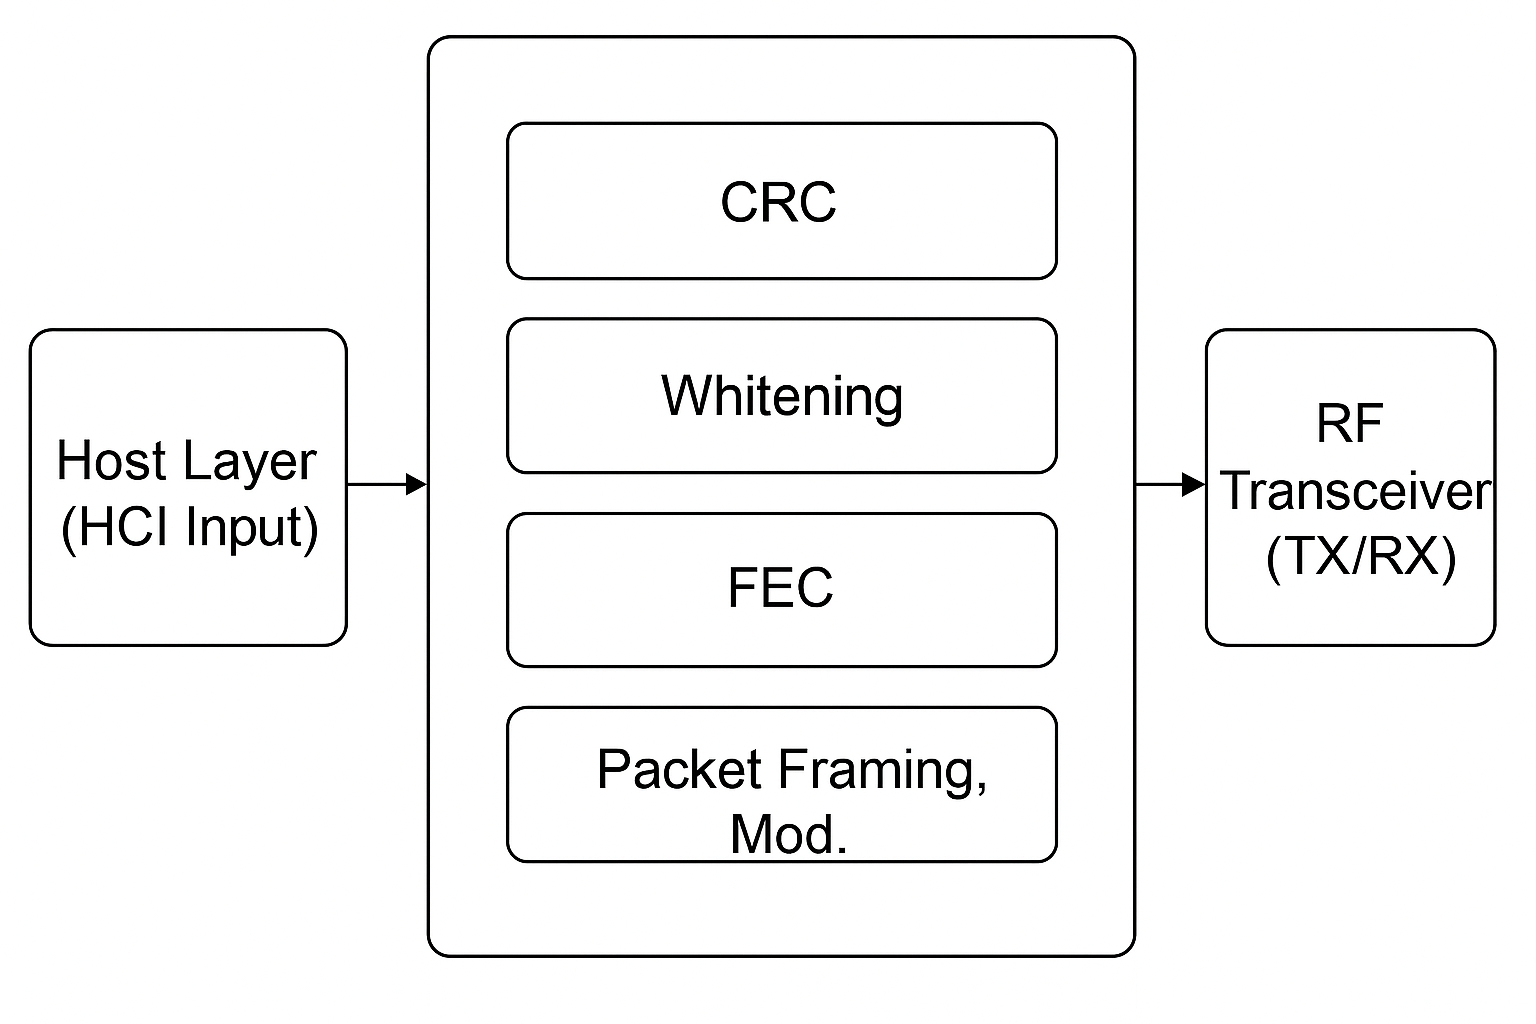
\includegraphics[width=0.8\textwidth]{ble_baseband_general_architecture.png}
\caption{Generalized block diagram of a Bluetooth Low Energy (BLE) digital baseband architecture highlighting common functional modules reviewed in literature.}
\label{fig:ble_general_architecture}
\end{figure}

\section{A Low-Power BLE Baseband Transmission Data Processing Module (2024)}
A low-power BLE baseband transmission data processing module based on Verilog
HDL was proposed by Liang Ding et al. (2024). The module comprised CRC generator,
data whitener, and FEC modules utilizing the concept of modularity. The simulation
test using Synopsys VCS proved functionality and low power consumption
capabilities. It was shown that the use of modularity in designing the baseband
system allows for better scalability and adherence to BLE 5.0 standards.

\section{A Baseband Processor for Impulse Ultra-Wideband Communications (2005)}
Blazquez et al. (2005) suggested a baseband processor design for impulse Ultra-Wide Band (UWB)
communication that uses 0.18\,$\mu$m CMOS technology. The baseband processor included a 4-bit,
1.2 Gsps Flash ADC, a Phase-Locked Loop (PLL), and digital synchronization circuits.
With the transfer of synchronization and correlation operations to the digital domain, the
4
architecture reduced the analog part of the circuitry. While intended for use in UWB,
the approach can be employed in the design of BLE baseband processors.

\section{A 10 mW Bluetooth Low-Energy Transceiver with On-Chip Matching (2016)}
In a paper titled “A Compact 10mW GFSK Modulated Bluetooth Low Energy Transceiver with Integrated Digital Baseband” published in 2016 by J.H. Lee et al., a 10mW BLE transceiver comprising both analog and digital baseband was discussed. In their design, impedance matching on chip, GFSK modulation technique, and integrated digital baseband were some notable features. It was shown that the optimization of both RF and baseband subsystems is highly beneficial for system performance.

\section{Comparison of Reviewed Works}
In general, all these papers show advances in the design of BLE baseband. Each paper concentrated on a specific area—energy efficiency, scalability, or integration. The following table shows the major findings and limitations of each paper.

\begin{table}[H]
\centering
\caption{Comparison of Reviewed Research Papers}
\label{tab:comparison}
\begin{tabular}{|c|p{4cm}|c|p{4cm}|p{4cm}|}
\hline
\textbf{Sr. No.} & \textbf{Title of Paper} & \textbf{Year} & \textbf{Benefits} & \textbf{Limitations} \\ \hline
1 & A Low-Power BLE Baseband Transmission Data Processing Module & 2024 & Efficient RTL design; includes CRC, whitening, and FEC modules; validated through simulation & Focused only on digital processing; lacks full-chip hardware realization \\ \hline
2 & A Baseband Processor for Impulse Ultra-Wideband Communications & 2005 & Fully digital synchronization; high-speed operation with scalable architecture & High power usage for BLE standards; not BLE-specific \\ \hline
3 & A 10 mW Bluetooth Low-Energy Transceiver with On-Chip Matching & 2016 & Integrated transceiver and baseband design; low-power operation suitable for IoT & Limited flexibility for custom baseband extensions \\ \hline
\end{tabular}
\end{table}





\chapter{Theoretical Background and Design Methodology}

\section{Theoretical Background}
Bluetooth low-energy (BLE) is a radio transmission system for short-range communication that consumes minimum power and is mainly used for transmitting data. The system utilizes a wireless frequency range known as the 2.4GHz Industrial, Scientific, and Medical (ISM) bands for effective data transmission with minimum energy loss. The system is popular because of its reliability, low price and efficient use in battery-powered gadgets.

Data transmitted via BLE communication involves packet-based transmission. BLE data packet consists of a synchronization sequence known as the preamble, an access address, a header, data payload, and a Cyclic Redundancy Check (CRC). The organization of data in packets guarantees reliable data transmission by making sure that data is structured properly before being sent out.

In order to ensure high-quality data transmission, BLE applies data whitening through Linear Feedback Shift Registers (LFSRs). BLE data transmission utilizes Gaussian Frequency Shift Keying (GFSK) modulation that transforms the digital signals to analog waveforms and thus reduces interference during transmission.

\begin{figure}[h]
    \centering
    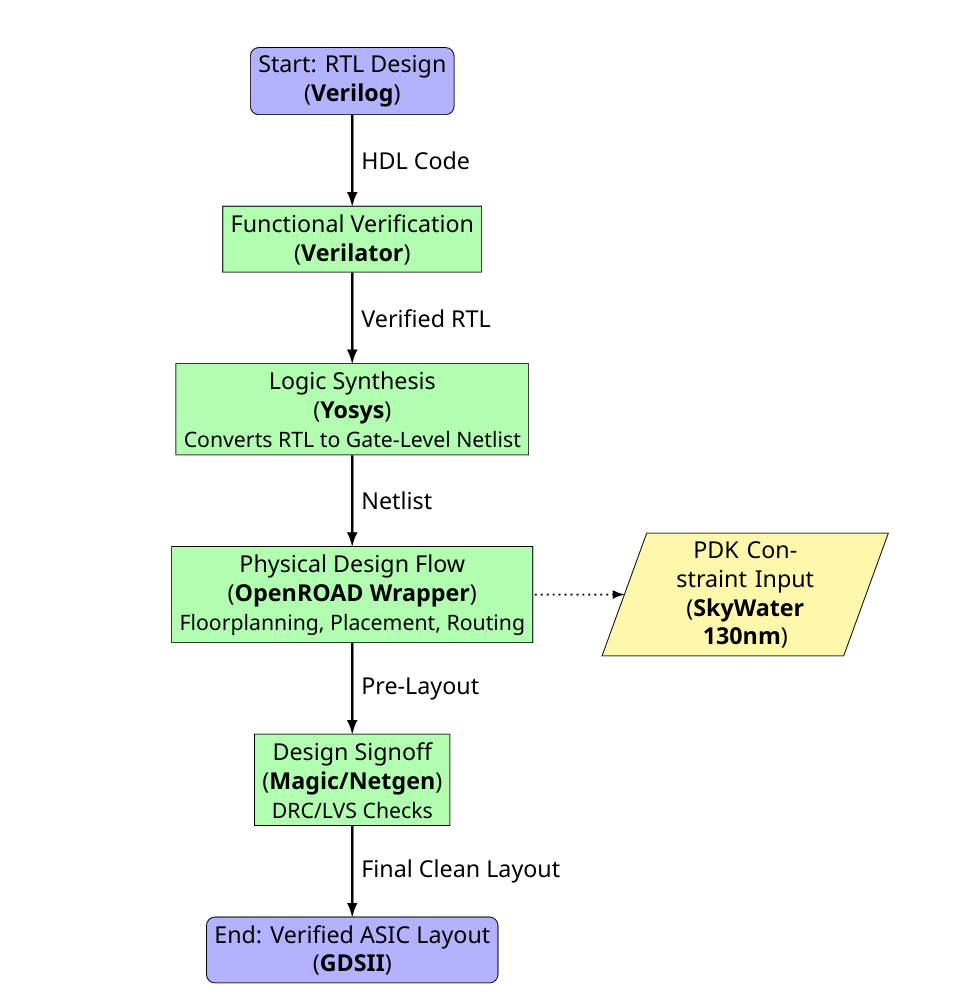
\includegraphics[width=0.7\textwidth]{flowchart.png}
    \caption{Process flow of BLE baseband processor.}
    \label{fig:flowchart}
\end{figure}

\section{Design Methodology}
The architecture uses the modular development concept for hardware, which starts with RTL coding,
then moves to simulation and verification. Modules are then tested individually before integrating the
system. BLE digital baseband processor has two major components namely transmitter path and receiver path.

\subsection{Transmitter Path}
\begin{figure}[H]
\centering
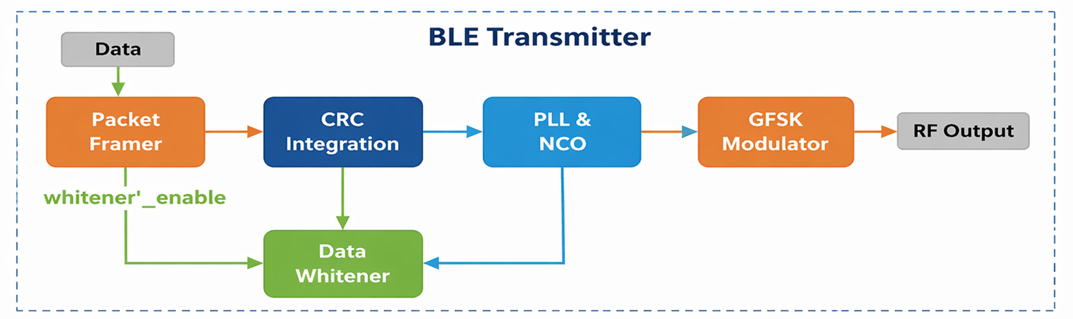
\includegraphics[width=0.9\textwidth]{image.png}
\caption{Transmitter path block diagram of the BLE digital baseband processor.}
\label{fig:tx_blockdiagram}
\end{figure}

Transmitter path converts the input data obtained through the Host Controller Interface (HCI)
into the RF data to be transmitted. The working mechanism of each module is explained in detail below:

\begin{itemize}
    \item \textbf{HCI Input:} The protocol data unit (PDU) from the higher-layer payloads is provided to the baseband layer through the HCI connection.
    \item \textbf{CRC-24 Generator:} Provides a 24-bit cyclic redundancy check using BLE polynomial to ensure data integrity.
    \item \textbf{Data Whitening:} The whitening function uses a 7-bit LFSR algorithm to avoid repetition of bits.
This also keeps the DC balance neutral.
    \item \textbf{Packet Framing:}  Adds synchronization bits, access address, and preamble to make the BLE packet frame and make it valid.
    \item \textbf{GFSK Modulator:} Modulates the digital packet frame and produces an FSK modulated signal to transmit via RF.
    \item \textbf{RF Transmitter:} This is responsible for transmitting the modulated data through the air interface.
\end{itemize}

\subsection{Receiver Path}
\begin{figure}[H]
\centering
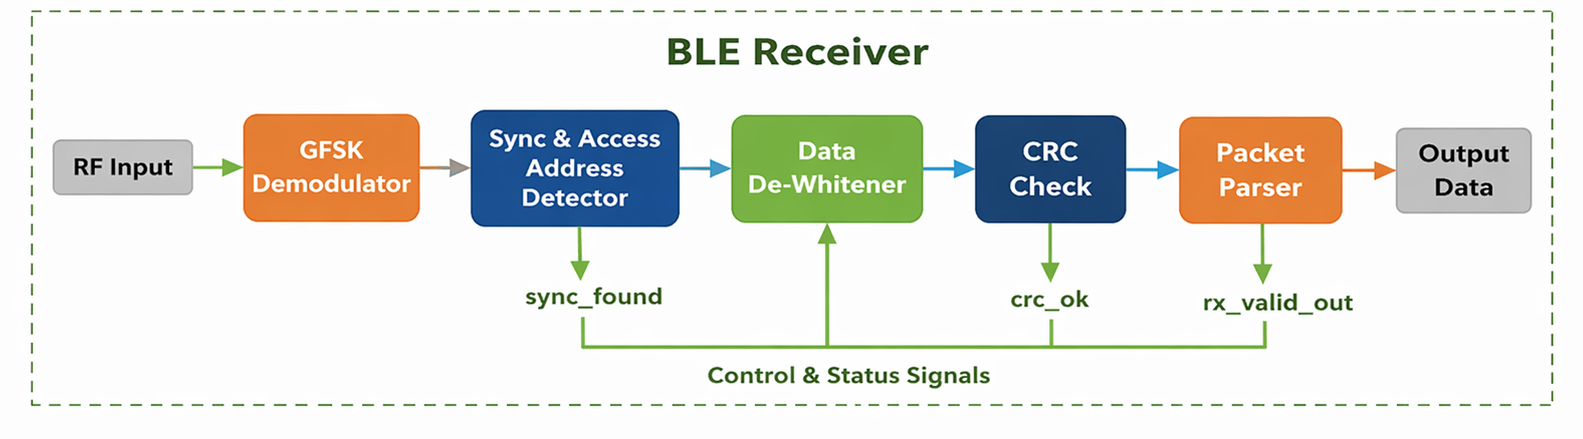
\includegraphics[width=0.9\textwidth]{image3.png}
\caption{Receiver path block diagram of the BLE digital baseband processor.}
\label{fig:rx_blockdiagram}
\end{figure}

The receiver’s operation does exactly the opposite of what transmitter does to retrieve information contained within the BLE signal, the individual blocks work as follows:

\begin{itemize}
    \item \textbf{RF Receiver:} Receives the incoming signal and demodulates it into the digital data stream.
    \item \textbf{GFSK Demodulator:} Extracts the information from the frequency-shifted keyed waveform using the process of demodulation.
    \item \textbf{Access Address and Sync Detector:} Recognizes the beginning of a BLE packet based on the presence of synchronization codes and access addresses.
    \item \textbf{Data De-Whitening:} Inverts the whitened signal by repeating the whitening process,
employing a 7-bit Galois Linear Feedback Shift Register (LFSR).
    \item \textbf{CRC-24 Checker:} Validates the CRC value against the actual value contained within the CRC field.
    \item \textbf{HCI Output:} Transmits the validated data to higher layers via the host controller interface.

The Hardware Interface of Transceiver is thoroughly specified in two important tables. The first table (Table 3.1) gives information on the highest level I/Os of the Open Core, which provides details about the connections related to power, clock, reset, and data buses. After that, the second table (Table 3.2) describes the pin specifications of various modules inside the transmitter, such as CRC-24 Generator, Packet Framer, Data Whitener, and GFSK Modulator.
\end{itemize}

% --- CODE FOR YOUR FIRST TABLE (e.g., Table 3.1) ---

\begin{longtable}{|p{2.5cm}|l|l|l|c|p{4.5cm}|}

    % --- CAPTION AND LABEL ---
    % This adds the name, number, and List of Tables entry
    \caption{Pin specifications for the OpenBLE-P1 Core.}
    \label{tab:ble_pins} \\

    % --- HEADER FOR THE *FIRST* PAGE ---
    \hline
    Block Name & Pin Name & Direction & Type & Size (bits) & Description \\ \hline
    \endfirsthead

    % --- HEADER FOR *ALL OTHER* PAGES ---
    % This will probably not be used for this short table,
    % but it's good practice.
    \multicolumn{6}{c}{\tablename\ \thetable{} -- Continued} \\ \hline
    Block Name & Pin Name & Direction & Type & Size (bits) & Description \\ \hline
    \endhead

    % --- FOOTER FOR THE *LAST* PAGE ---
    \hline
    \endlastfoot

    % --- YOUR TABLE DATA ---
    Open Core & VDD, VSS & Input & Power & 1 & Power (1.8V) and Ground connections. \\ \hline
    ~ & clk & Input & Logic & 1 & Master clock input (Target: 20 MHz). \\ \hline
    ~ & rst\_n & Input & Logic & 1 & Active-low asynchronous reset. \\ \hline
    ~ & tx\_data\_in & Input & Bus & 8 & 8-bit bus to load transmit payload data. \\ \hline
    ~ & tx\_valid\_in & Input & Logic & 1 & Indicates tx\_data\_in is valid (handshake). \\ \hline
    ~ & start\_tx & Input & Logic & 1 & Pulse to begin a transmission. \\ \hline
    ~ & demod\_in & Input & Logic & 1 & Single-bit input from the ADC/RF front-end. \\ \hline
    ~ & tx\_ready\_out & Output & Logic & 1 & Indicates core is ready for new transmit data. \\ \hline
    ~ & rx\_data\_out & Output & Bus & 8 & 8-bit bus for received payload data. \\ \hline
    ~ & rx\_valid\_out & Output & Logic & 1 & Indicates valid data is on rx\_data\_out. \\ \hline
    ~ & irq\_tx\_done  & Output & Logic & 1 & Interrupt indicating transmission is complete. \\ \hline
    ~ & irq\_rx\_done & Output & Logic & 1 & Interrupt indicating a packet has been received. \\ \hline
    ~ & modulated\_out & Output & Logic & 1 & Single-bit modulated GFSK output to DAC. \\

\end{longtable}
% Preamble must have: \usepackage{longtable}

% --- START OF THE LONG TABLE ---
% I have changed ALL columns to p{...} (paragraph) type.
% This forces text to wrap in every column, solving the width problem.
% You can "tweak" these widths (e.g., p{2.5cm}) to your liking.

\begin{longtable}{|p{2.5cm}|p{3cm}|p{1.5cm}|p{1.5cm}|p{1.2cm}|p{4.5cm}|}

% --- CAPTION AND LABEL ---
\caption{Pin specifications for Transmitter Sub-blocks.}
\label{tab:tx_sub_blocks} \\

% --- HEADER FOR THE *FIRST* PAGE ---
\hline
Block Name & Pin Name & Direction & Type & Size (bits) & Description \\ \hline
\endfirsthead

% --- HEADER FOR *ALL OTHER* PAGES ---
% This automatically repeats the header on page 2, 3, etc.
\multicolumn{6}{c}{\tablename\ \thetable{} -- Continued} \\ \hline
Block Name & Pin Name & Direction & Type & Size (bits) & Description \\ \hline
\endhead

% --- FOOTER FOR THE *LAST* PAGE ---
% This puts a line at the very end of the table.
\hline
\endlastfoot

% --- YOUR TABLE DATA GOES HERE ---
CRC-24 Generator & clk & Input & Logic & 1 & Master clock signal. \\ \hline
~ & rst\_n & Input & Logic & 1 & Active-low asynchronous reset. \\ \hline
~ & enable & Input & Logic & 1 & Enables the register to process one bit. \\ \hline
~ & data\_in & Input & Logic & 1 & A single serial data bit from the PDU. \\ \hline
~ & crc\_out & Output & Bus & 24 & The final parallel CRC value after processing. \\ \hline
Packet Framer & clk & Input & Logic & 1 & Master clock signal. \\ \hline
~ & rst\_n & Input & Logic & 1 & Active-low asynchronous reset. \\ \hline
~ & start\_tx & Input & Logic & 1 & Single-cycle pulse to begin transmission. \\ \hline
~ & tx\_data\_in & Input & Bus & 8 & Parallel payload data from the host CPU. \\ \hline
~ & tx\_valid\_in & Input & Logic & 1 & Handshake signal indicating tx\_data\_in is valid. \\ \hline
~ & crc\_in & Input & Bus & 24 & The completed CRC value from the CRC block. \\ \hline
~ & tx\_ready\_out & Output & Logic & 1 & Handshake signal indicating it's ready for data. \\ \hline
~ & irq\_tx\_done & Output & Logic & 1 & Interrupt signaling that transmission is complete. \\ \hline
~ & crc\_enable & Output & Logic & 1 & Internal control signal to enable the CRC block. \\ \hline
~ & whitener\_enable & Output & Logic & 1 & Internal control signal to enable the Whitener. \\ \hline
~ & channel\_ind\_out & Output & Bus & 6 & The 6 bits that tell the data whitener the channel \\ \hline
~ & serial\_data\_out & Output & Logic & 1 & Serialized data going to the Whitener. \\ \hline
Data Whitener & clk & Input & Logic & 1 & Master clock signal. \\ \hline
~ & rst\_n & Input & Logic & 1 & Active-low asynchronous reset. \\ \hline
~ & enable & Input & Logic & 1 & Enables the whitening operation on data\_in. \\ \hline
~ & data\_in & Input & Logic & 1 & A single serial data bit from the Framer. \\ \hline
~ & channel\_index & Input & Bus & 6 & 6 digit channel number \\ \hline
~ & whitened\_data\_out & Output & Logic & 1 & The scrambled output data bit. \\ \hline
GFSK Modulator & clk & Input & Logic & 1 & Master clock signal. \\ \hline
~ & rst\_n & Input & Logic & 1 & Active-low asynchronous reset. \\ \hline
~ & data\_in & Input & Logic & 1 & The whitened data bit from the Whitener. \\ \hline
~ & modulated\_out & Output & Logic & 1 & Final single-bit modulated output for the DAC. \\

% --- END OF THE LONG TABLE ---
\end{longtable}
\section{CRC Generation and Data Whitening Logic}
The CRC and data whitening modules constitute the fundamental blocks of the digital baseband scheme.
Both are realized by means of LFSRs, providing an efficient implementation for the
serial processing of bits.

\subsection{CRC Generation using Fibonacci LFSR}
Cyclic Redundancy Check (CRC)
Error detection can be done through cyclic redundancy check (CRC). This algorithm uses polynomial division to detect errors in the data stream. The output from this operation is the CRC code.
Fibonacci LFSR hardware design
Figure 3.4 shows a 4-bit Fibonacci LFSR implementation that explains how the process works. In this setup, the flip-flop acts as the bits of the CRC code. The XOR logic gate indicates the feedback path.
According to the Bluetooth Low Energy (BLE) protocol, a 24-bit LFSR hardware structure will be employed to generate the CRC code based on the following polynomial:
\[
P(x) = x^{24} + x^{10} + x^9 + x^6 + x^4 + x^3 + x + 1
\]
The extended 24-bit design follows similar logic to that exhibited in the 4-bit example,
where additional registers and feedback taps are placed in relevant locations, as dictated by the polynomial. This helps in the proper identification of errors within the BLE packets.

\subsection{Data Whitening using Galois LFSR}
Whitening of data enhances the reliability of signal by avoiding repetitive strings of
identical bits that might result in synchronization or DC offset errors. The whitening is
done through a Galois LFSR arrangement, which uses parallel feedback for quick processing.
A 4-bit Galois design depicted in Figure 3.4 provides an insight into the underlying principle.
Here, the XOR feedback alters several output values from flip flops, thus creating a random bit
sequence.
In Bluetooth Low Energy, a 7-bit Galois LFSR based on the following polynomial:
\[
P(x) = x^7 + x^4 + 1
\]
is utilized in the process of whitening. The reasoning follows the same route as
that of the 4-bit configuration, except that more stages are added, and feedback taps
are located on bits 7 and 4. Whitening is accomplished during transmission by
XORing the bit stream with the sequence generated.

\begin{figure}[H]
\centering
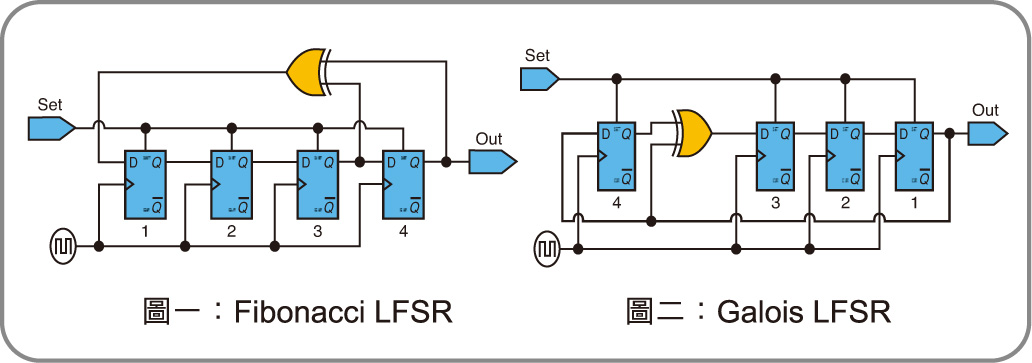
\includegraphics[width=0.9\textwidth]{lfsr_fibonacci_galois.jpg}
\caption{4-bit Fibonacci and Galois Linear Feedback Shift Register (LFSR) models used for CRC generation and data whitening respectively.}
\label{fig:lfsr_models}
\end{figure}

\section{GFSK Modulation}
Gaussian Frequency Shift Keying (GFSK) is the modulation technique used in BLE for transmitting data. It converts digital bits into frequency variations, where different frequencies represent binary `0' and `1'. A Gaussian filter is applied before modulation to smooth the signal transitions and reduce bandwidth. This improves spectral efficiency and minimizes interference with other signals in the channel.

\section{GFSK Demodulation}
GFSK demodulation is the process of recovering digital data from the received modulated signal. It detects frequency shifts in the incoming signal and converts them back into binary data. This process reverses the modulation operation performed at the transmitter. Accurate demodulation is essential for correct data recovery.

\section{De-Whitening}
De-whitening is performed at the receiver to restore the original data sequence. It uses the same Linear Feedback Shift Register (LFSR) configuration as used during data whitening. This ensures that the randomized data is converted back to its original form. Proper synchronization of the LFSR is necessary for correct de-whitening.

\section{Packet Structure and Parsing}
BLE communication uses a structured packet format for data transmission. Each packet includes a preamble, access address, header, payload, and CRC. At the receiver, the packet parser identifies and extracts these fields based on predefined positions. This allows correct interpretation and processing of the received data.

\section{CRC and Error Detection}
Cyclic Redundancy Check (CRC) is used for error detection in BLE communication. A CRC value is generated at the transmitter and appended to the packet. At the receiver, the CRC is recalculated and compared with the received value. If both values match, the data is considered valid; otherwise, it is rejected.

\section{Receiver Operation}
The receiver performs multiple operations to recover the transmitted data. It first demodulates the received signal to obtain the bitstream. The data is then de-whitened and passed to the packet parser. Finally, CRC verification ensures the correctness of the received data.

\section{GFSK Calculations}

Gaussian Frequency Shift Keying (GFSK) is used in BLE to convert digital data into smooth frequency variations, ensuring reduced bandwidth and continuous phase.

\subsubsection{Frequency Deviation}

The frequency deviation ($\Delta f$) is derived from modulation index $h$ and bit duration $T_b$:

\begin{equation}
h = (2\Delta f)\cdot T_b
\end{equation}

\begin{equation}
\Delta f = \frac{h}{2T_b}
\end{equation}

For BLE, $h = 0.5$ and $T_b = 1 \,\mu s$:

\begin{equation}
\Delta f = 250 \, \text{kHz}
\end{equation}

---

\subsubsection{Input Data Representation}

The binary input sequence is represented as:

\begin{equation}
x(t) = \sum_i a_i \delta(t - iT_b)
\end{equation}

where $a_i \in \{+1, -1\}$.

---

\subsubsection{Gaussian Filter (Time Domain)}

The Gaussian impulse response is:

\begin{equation}
g(t) = \frac{1}{\sqrt{2\pi}\sigma} e^{-\frac{t^2}{2\sigma^2}}
\end{equation}

---

\subsubsection{Gaussian Filter (Frequency Domain)}

Applying Fourier Transform:

\begin{equation}
G(f) = e^{-2\pi^2 \sigma^2 f^2}
\end{equation}

This limits high-frequency components and reduces spectral width.

---

\subsubsection{Inverse Fourier Transform}

\begin{equation}
g(t) = \int_{-\infty}^{\infty} G(f) e^{j2\pi ft} df
\end{equation}

---

\subsubsection{Convolution with Input Data}

The filtered signal is obtained by convolution:

\begin{equation}
s(t) = x(t) * g(t)
\end{equation}

\begin{equation}
s(t) = \sum_i a_i g(t - iT_b)
\end{equation}

This smooths sharp transitions in the input signal.


\subsubsection{Instantaneous Frequency}

\begin{equation}
f(t) = s(t)
\end{equation}


\subsubsection{Phase Calculation}

The phase is obtained by integrating frequency:

\begin{equation}
\theta(t) = 2\pi h \int_{-\infty}^{t} s(\tau) d\tau
\end{equation}

\begin{equation}
\theta(t) = 2\pi h \sum_i a_i \int_{-\infty}^{t} g(\tau - iT_b) d\tau
\end{equation}

This ensures continuous phase modulation.


\section{PLL and Phase Accumulator Calculations}

\subsubsection{PLL Frequency Scaling}

\begin{equation}
M = \frac{F_{int}}{F_{ref}} = \frac{400 \, \text{MHz}}{20 \, \text{MHz}} = 20
\end{equation}

Thus, internal clock:

\begin{equation}
F_{int} = 400 \, \text{MHz}
\end{equation}

---

\subsubsection{Samples Per Symbol}

\begin{equation}
SPS = \frac{F_{int}}{R}
\end{equation}

For $R = 20 \, \text{Mbps}$:

\begin{equation}
SPS = 20
\end{equation}



\subsubsection{NCO Tuning Word Calculation}

The tuning word for NCO:

\begin{equation}
M = \frac{F_{target} \cdot 2^N}{F_{int}}
\end{equation}

For $N = 8$:

\textbf{Carrier Frequency:}

\begin{equation}
M_{center} = 64
\end{equation}

\textbf{Frequency Deviation:}

\begin{equation}
M_{dev} \approx 6.4 \approx 6
\end{equation}



\subsubsection{Frequency Mapping}

\begin{itemize}
\item Logic `1' $\rightarrow 64 + 6 = 70$
\item Logic `0' $\rightarrow 64 - 6 = 58$
\end{itemize}



\subsubsection{Phase Accumulator Operation}

\begin{equation}
\theta[n] = \theta[n-1] + M
\end{equation}

This performs discrete integration of frequency and ensures phase continuity.



\subsubsection{Clock Timing}

\begin{equation}
T = \frac{1}{400 \, \text{MHz}} = 2.5 \, \text{ns}
\end{equation}

\begin{equation}
T_{toggle} = 1.25 \, \text{ns}
\end{equation}


\subsubsection{Verification from Simulation}

\begin{itemize}
\item External Clock = 20 MHz
\item Internal Clock = 400 MHz
\item RF Output (Logic 1) $\approx 106$ MHz
\item RF Output (Logic 0) $\approx 93$ MHz
\end{itemize}

These results confirm correct implementation of GFSK modulation.

\section{Summary}

The theoretical basis of the BLE baseband transceiver was provided in this chapter. The basics of BLE communication, such as packet, the data whitening technique using LFSR, and GFSK modulation and demodulation processes were discussed in detail.

Moreover, mathematical and system level calculations for the design process were carried out. The frequency deviation and phase generation equations for GFSK were derived for continuous phase modulation. The use of the PLL for frequency scaling and the process of the phase generation using the phase accumulator in the NCO(Numerical Control Oscillator) were provided. All these together form the connection between theoretical modeling and RTL design.

Generally, this chapter has provided sufficient information on the BLE baseband system and served as a good theoretical basis for the design described in the next chapters.



\chapter{Software Used and Simulation Results}

\section{Software Tools Used}
The design and verification of the BLE digital baseband processor were done using open-source Electronic Design Automation (EDA) tools. Each software has its unique role in the hardware design process.

\begin{itemize}
    \item \textbf{Iverilog:} Verilog compiler that is used to verify the functionality of HDL modules.
    \item \textbf{Yosys:} Converts Verilog RTL code into gate-level netlist and optimizes logic for minimum area and maximum speed.
    \item \textbf{OpenROAD:} Place and route tool that optimizes timings.

    \item \textbf{Magic:} Checks DRC(Design Rule Check) rules and exports the final GDSII layout for manufacturing.
    \item \textbf{Netgen:} Executes and Validates the netlist and layout through LVS(Layout-Versus-Schematic).
    \item \textbf{Verilator:} Simulator for high-speed verification and linting of Verilog code.
    \item \textbf{KLayout:} Graphical viewer used for inspection and validation of GDSII layout files.
\end{itemize}
\usepackage{float} % add this in preamble

\section{Simulation Results}

The output from the simulation confirms that the design is working perfectly fine. For testing purposes, an input message is taken and the performance of both transmitter and receiver sections of the BLE baseband transceiver is investigated.

\subsubsection{Transmitter Waveform:}
\begin{figure}[H]
\centering
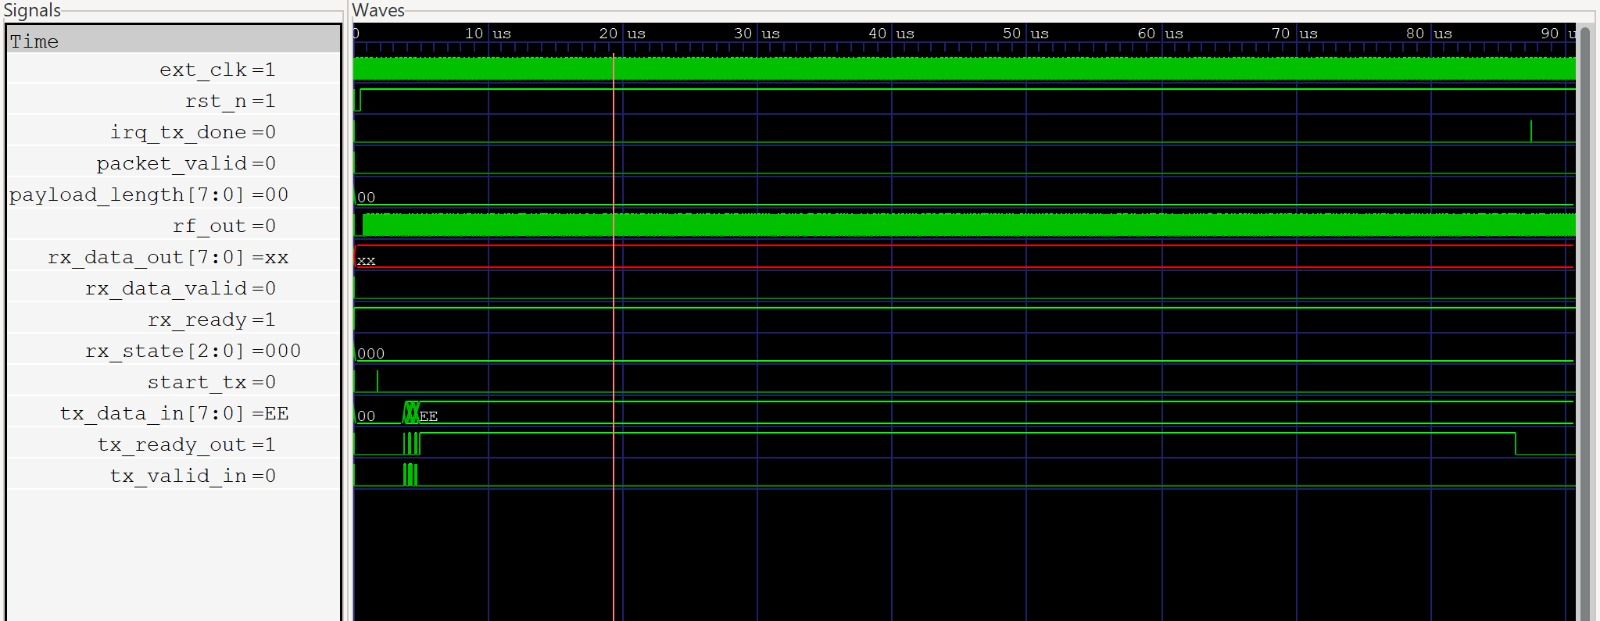
\includegraphics[width=0.9\linewidth]{tx_waveform.png}
\caption{Transmitter Simulation Waveform}
\end{figure}

The waveform from the transmitter represents the creation of a whole BLE data packet. This is evident from the inclusion of the preamble, access address, header, payload, and CRC in the signal.

\subsubsection{Receiver Waveform:}
\begin{figure}[H]
\centering
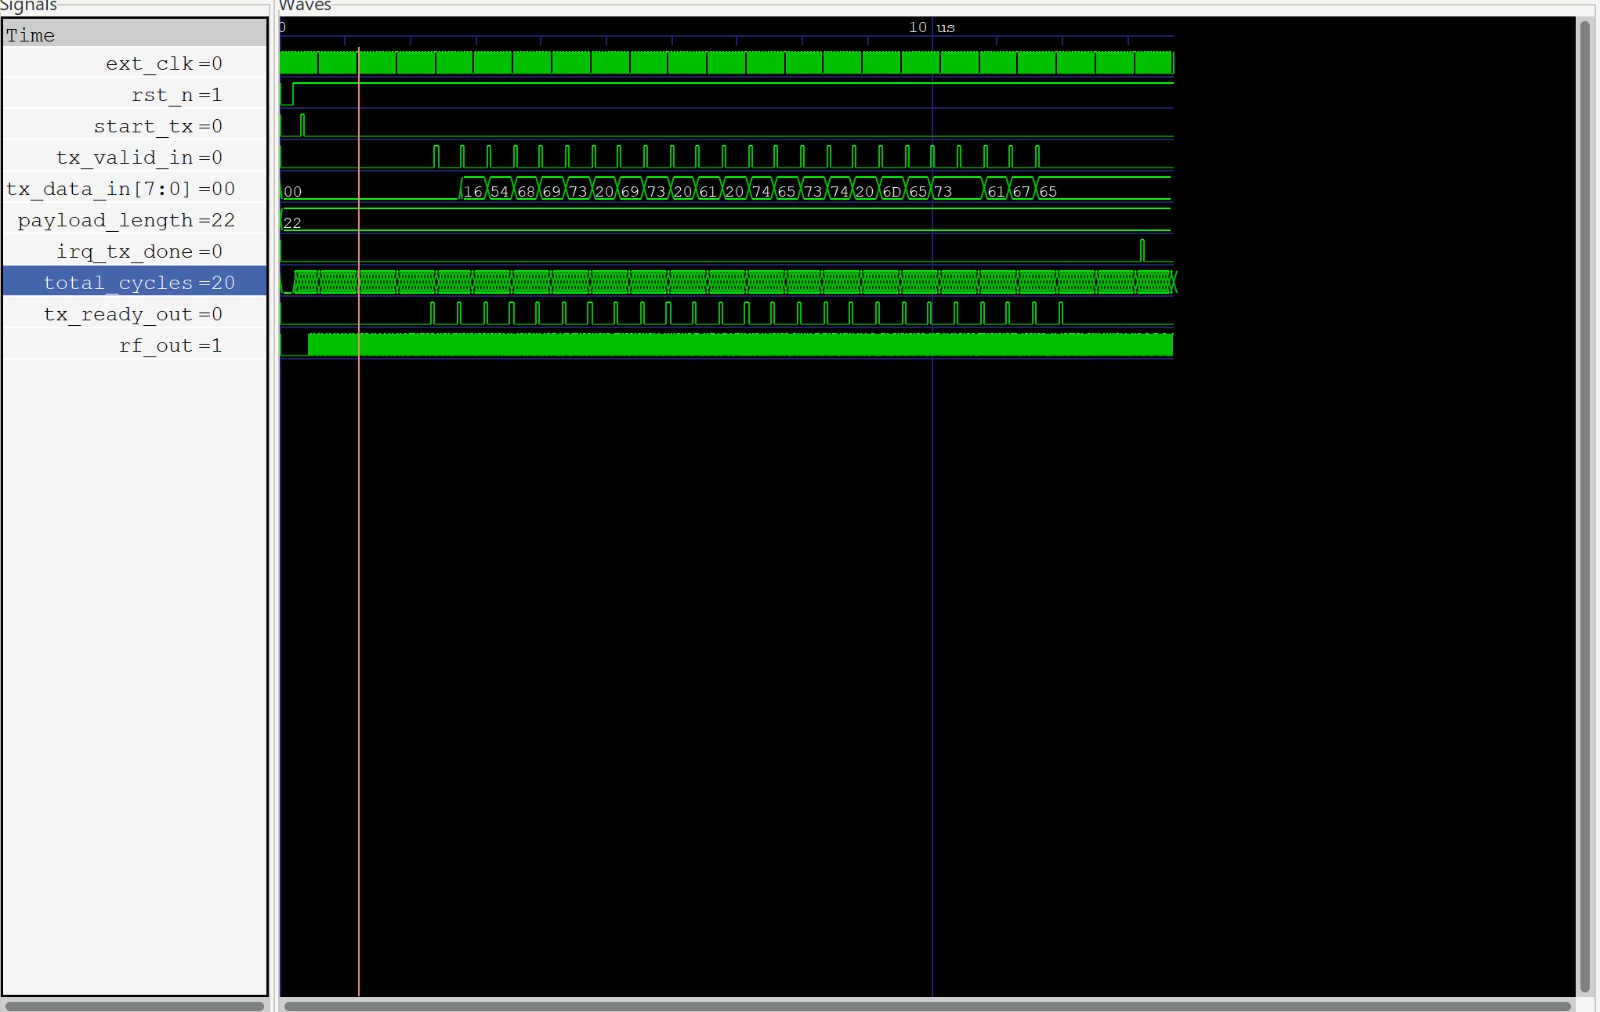
\includegraphics[width=0.9\linewidth]{rx_waveform.png}
\caption{Receiver Simulation Waveform}
\end{figure}

The demodulated waveform proves the accuracy of the demodulation process along with data retrieval. The data de-whitening and packets parsing modules perform extraction of transmitted data successfully.

\subsubsection{Terminal Output Result:}
\begin{figure}[H]
\centering
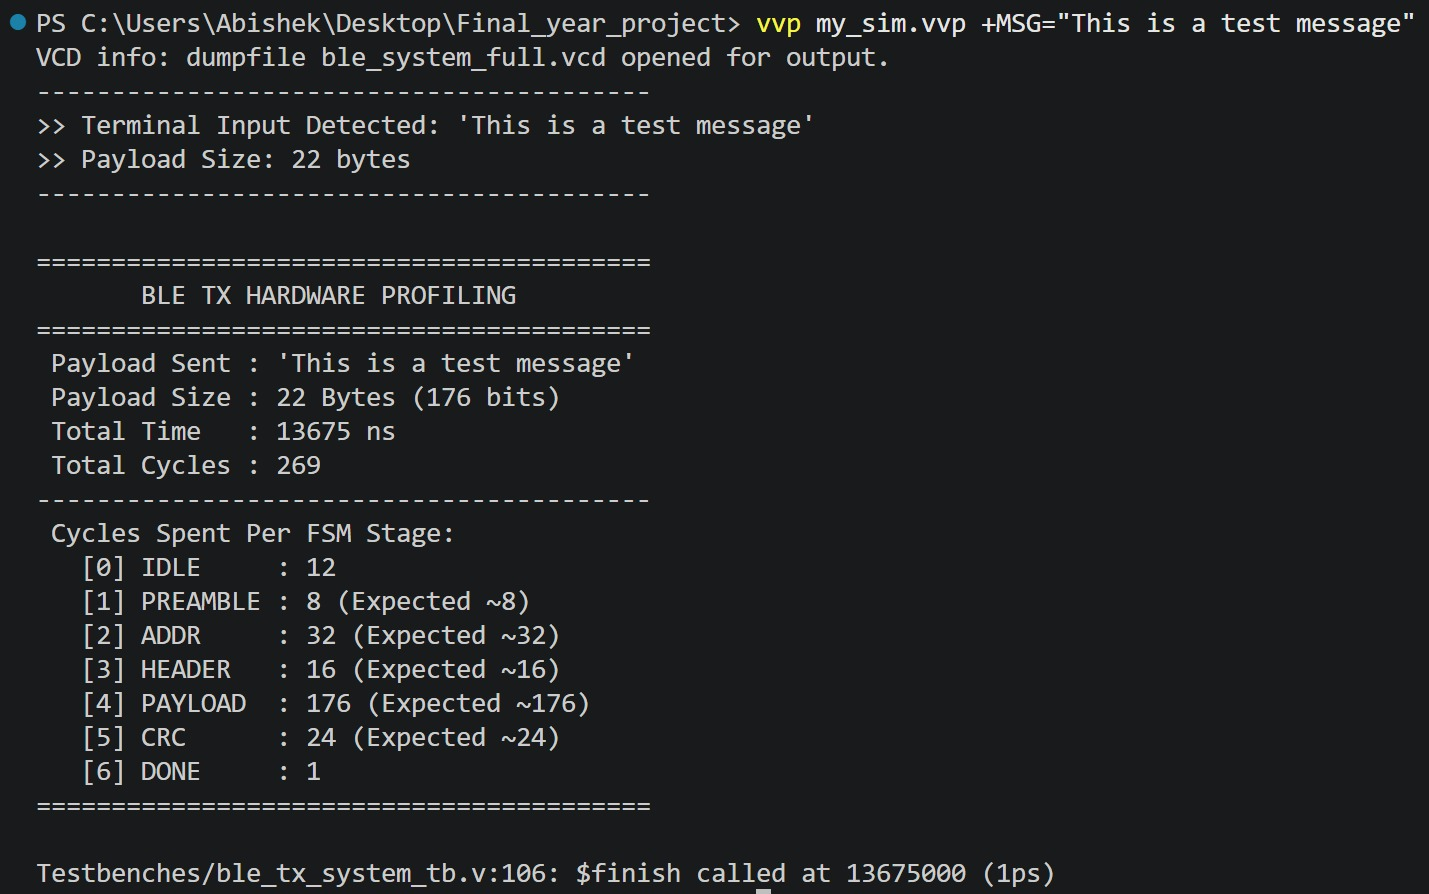
\includegraphics[width=0.9\linewidth]{terminal_output.png}
\caption{Simulation Terminal Output}
\end{figure}

Output from the terminal demonstrates the processing of the input string “This is a test message” by the system. This includes the payload size, total number of cycles, and state-machine execution of the system per stage. The output proves that packets were successfully transmitted, 24-bit CRC was generated, and transmission completed successfully.
\hypersetup{
    colorlinks=true,
    urlcolor=blue,
    linkcolor=black,
    citecolor=black
}

\chapter{Conclusion and Future Scope}

\section{Conclusion}
Designing and simulating of a BLE digital baseband transceiver has been successfully accomplished using Verilog HDL. The system performed critical baseband functionalities like packet generation, data whitening, GFSK modulation, demodulation, de-whitening, packet decoding, and error detection using 24-bit cyclic redundancy checks. The successful simulation confirmed that the transmitted data was correctly received at the other end through proper synchronization and data verification. This project gives an insight into how BLE communication is done internally and provides an excellent platform to understand the designing of a wireless system.

\section{Future Scope}
However, the design is currently confined to the simulation of the baseband block alone. For future studies, this design can be extended to include its implementation using FPGA technology to test its real-world performance. Its connection to the RF front end will help realize wireless communication fully. There are several ways through which power efficiency can be improved, and there can also be other additions like channel hopping and multiple nodes communication.



\chapter*{References}
\addcontentsline{toc}{chapter}{References}

\begin{small}
\sloppy
\begin{enumerate}

\item N. Sharma and R. Kumar, “Design of Low-Power BLE Transceiver for IoT Applications,” \textit{E3S Web of Conferences (VESSEP 2023)}, vol. 404, pp. 1--5, 2023. [Online]. Available: \url{https://doi.org/10.1051/e3sconf/202340401044}

\item C. Su and M. Lee, “A 10~mW Bluetooth Low-Energy Transceiver with On-Chip Matching,” \textit{IEEE Journal of Solid-State Circuits}, vol. 56, no. 3, pp. 830--841, Mar.~2021. [Online]. Available: \url{https://doi.org/10.1109/JSSC.2020.3036432}

\item R. Blazquez, F. P. de Gyvez, R. D. Struik, and J. Pineda, “A 2.4~GHz Bluetooth Transceiver for Low-Power Wireless Communications,” \textit{IEEE Journal of Solid-State Circuits}, vol. 40, no. 2, pp. 474--482, Feb.~2005. [Online]. Available: \url{https://doi.org/10.1109/JSSC.2004.839503}

\item Bluetooth Special Interest Group, “Bluetooth Core Specification Version~5.4,” Feb.~2023. [Online]. Available: \url{https://www.bluetooth.com/specifications/bluetooth-core-specification/}

\item C. Gomez and J. Paradells, “Overview and Evaluation of Bluetooth Low Energy: An Emerging Low-Power Wireless Technology,” \textit{Sensors}, vol. 12, no. 9, pp. 11734--11753, 2012. [Online]. Available: \url{https://doi.org/10.3390/s120911734}

\item P. Kindt, D. Yunge, R. Diemer, and S. Chakraborty, “Precise Energy Modeling for the Bluetooth Low Energy Protocol,” \textit{arXiv preprint arXiv:1403.2919}, Mar.~2014. [Online]. Available: \url{https://arxiv.org/abs/1403.2919}

\item S. Hosni, T. Zaki-Abdellatif, I. Siouane, and Y. Askouri, “Bluetooth Low Energy: A Survey,” \textit{International Journal of Computer Applications}, vol. 162, no. 1, pp. 10--18, Mar.~2017. [Online]. Available: \url{https://doi.org/10.5120/ijca2017913248}

\item B. Pang, X. Liu, B. Li, J. Yang, and Z. Tang, “Bluetooth Low Energy Interference Awareness Scheme,” \textit{Sensors}, vol. 21, no. 7, p. 2257, Apr.~2021. [Online]. Available: \url{https://doi.org/10.3390/s21072257}

\item S. Sridhar, P. Misra, G. S. Gill, and J. Warrior, “CheepSync: A Time Synchronization Service for Resource-Constrained Bluetooth Low Energy Advertisers,” \textit{arXiv preprint arXiv:1501.06479}, Jan.~2015. [Online]. Available: \url{https://arxiv.org/abs/1501.06479}

\item M. Kolakowski, “Kalman Filter Based Localization in Hybrid BLE-UWB Positioning System,” \textit{arXiv preprint arXiv:2404.02349}, Apr.~2024. [Online]. Available: \url{https://arxiv.org/abs/2404.02349}

\item Bluetooth SIG, “The Bluetooth Low Energy Primer Version~1.2,” Mar.~2024. [Online]. Available: \url{https://www.bluetooth.com/wp-content/uploads/2022/05/the-bluetooth-le-primer-v1.2.0.pdf}

\end{enumerate}
\end{small}





%\chapter*{Publications} 
%\addcontentsline{toc}{chapter}{\textbf{Publications}}
%{\large \bf Conference Publications}
%{\textbf{\large{Conference Publications:}}}
%\begin{enumerate}

	%---------------------------------------------------------
%	\item[(1)]  
	
	                                                               
%\end{enumerate}



\appendix
\clearpage
\section*{Appendix A: Project Timeline Chart}
\addcontentsline{toc}{section}{Appendix A: Project Timeline Chart}

\begin{figure}[H]
    \centering
    % Replace the filename below with your actual file name if different
    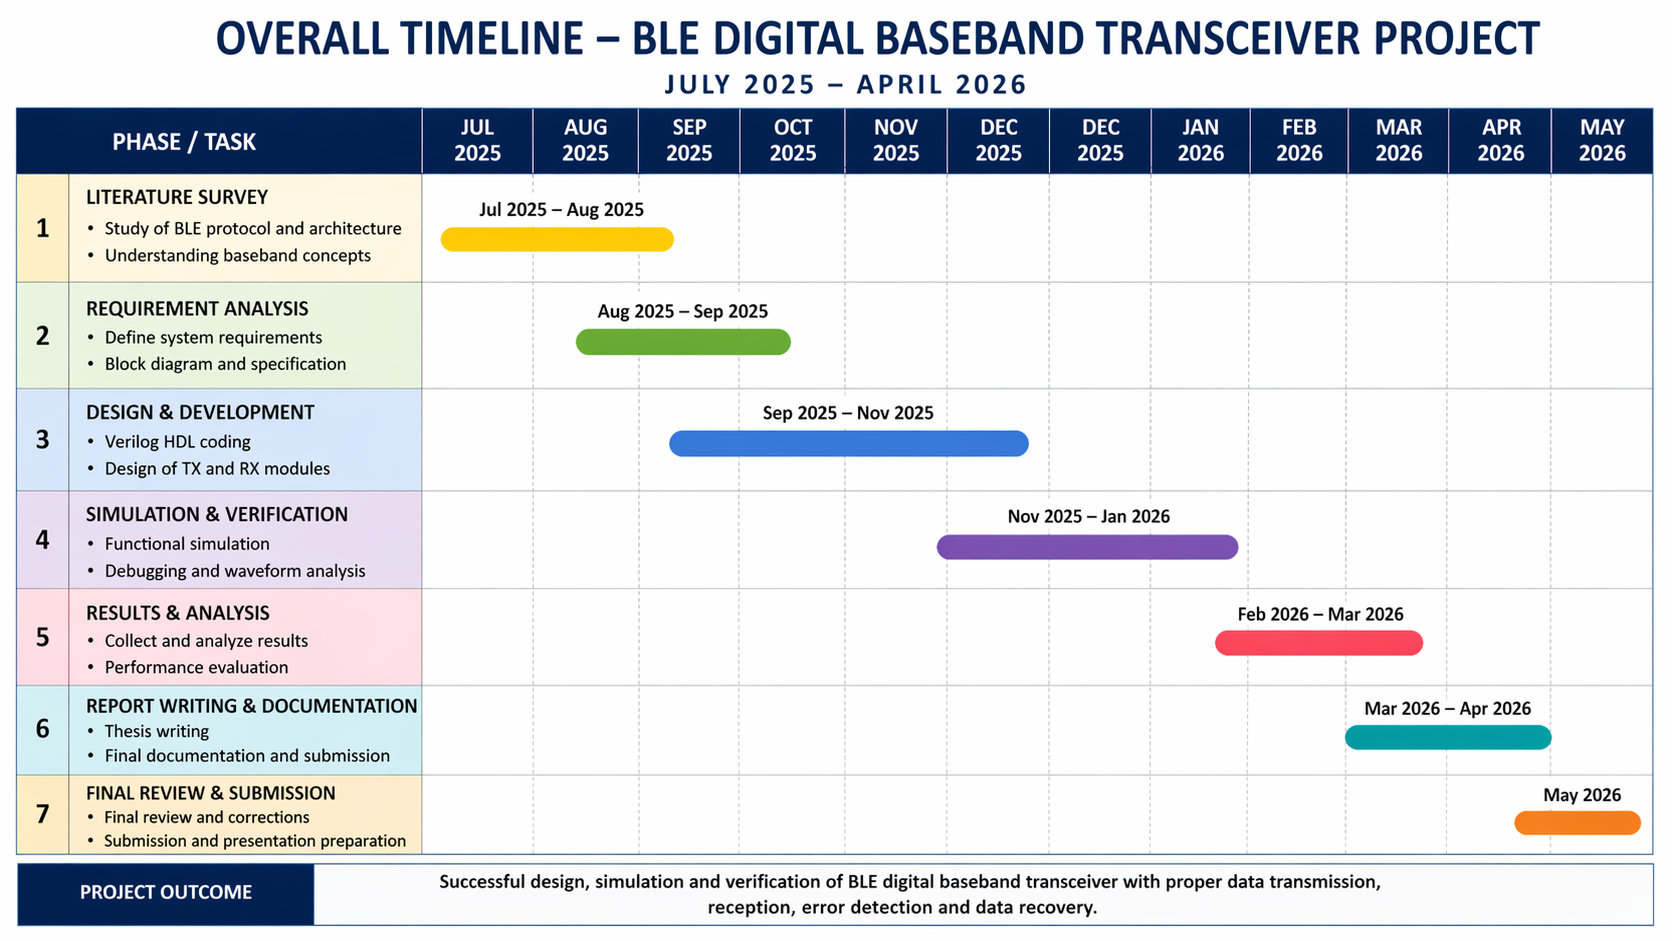
\includegraphics[width=\textwidth,height=0.5\textheight,keepaspectratio]{timechart.png}
    \caption*{\textbf{Overall Timeline of VLSI Based BLE Digital Baseband Transceiver Project (July 2025 – April 2026)}}
\end{figure}

\vspace{6pt}


\end{appendices}

\end{document}

